\documentclass[a4paper,12pt]{article}

\usepackage{amsmath,amssymb,amsthm,tikz}
\usetikzlibrary{calc,arrows.meta}
\usepackage[margin=20mm]{geometry}
\usepackage{hyperref}

\setlength{\parindent}{0pt}
\setlength{\columnsep}{1cm}

\begin{document}

\twocolumn

\thispagestyle{empty}

\begin{center}
{\Large Assignment 13}\\
{\Large Published on 2020-12-06,}\\
{\em Estimated Time: 30 minutes,}\\
{\em Max.grade 10\textperthousand} 
\end{center}


\section{Dijkstra's Algorithm}

(Goodrich2011, p.640) defines Dijkstra's algorithm. 
See also \url{https://bit.ly/2JSXqMU}. 
It is an efficient algorithm; it requires $O((m+n)\log_2 n)$ time, if 
we use priority queues; here $m$ is the number of edges and $n$ is the number 
of vertices in a graph.
 
In this exercise you do not need to implement a priority queue; 
assume that you can always pick the vertex with the smallest distance and 
add it to the set $S$ of visited vertexes (those having distances already computed). 



\section{Problem}

We start with the graph shown in Figure~\ref{fig:problem-graph}.

\begin{figure}[!htb]
\center{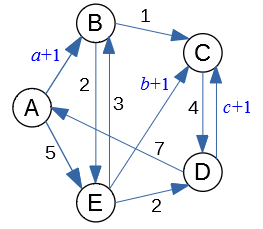
\includegraphics[width=2in]{assignment13-dijkstra/problem-graph.png}}
\caption{\label{fig:problem-graph} Graph diagram}
\end{figure}

The following edges $(A,B)$, $(E,C)$, $(D,C)$ have weights 
$a+1$, $b+1$, and $c+1$ respectively 
(here $a,b,c$ should be replaced by the digits from your Student ID). 
Vertex $A$ will be your source vertex. (You can assume that the distance 
from $A$ to itself is $0$; initially all the other distances are infinite, but 
then Dijkstra's algorithm relaxes them). 


\vspace{10pt}
{\bf (A)} Redraw the graph Figure~\ref{fig:problem-graph}, 
replace the edge weights $a+1$, $b+1$, and $c+1$ by your values of $a,b,c$. 


\vspace{10pt}
{\bf (B)} Run the Dijkstra's algorithm; 
create a table showing how distances to $A,B,C,D,E$ 
change as the relaxations are performed.
At every iteration highlight which vertex (among those not yet finished) 
has the minimum distance. Add it to the set $S$ of finished vertices 
(the set $S$ will have $0$ in the very first iteration; after that it will grow by 
one vertex at a time). 

\vspace{10pt}
{\bf (C)} Summarize the result: For each of the $5$ vertices 
tell what is its minimum distance from the source. 
Also tell what is the shortest path how to get there. 

\end{document}

